\chapter{Anode Plane Assemblies}
\label{ch:fdsp-apa}

%%%%%%%%%%%%%%%%%%%%%%%%%%%%%%%%%%%%%%%%%%%%%%%%%%%%%%%%%%%%%%%%%%%%
\section{Anode Plane Assembly (APA) Overview}
\label{sec:fdsp-apa-ov}

%%%%%%%%%%%%%%%%%%%%%%%%%%%%%%%%%%%%%
\subsection{Introduction}
\label{sec:fdsp-apa-intro}

Anode Plane Assemblies (APAs) are the far detector elements utilized to sense ionization created by
charged particles traversing the liquid argon volume inside the single-phase TPC. The planes are interleaved with Cathode Plane Assemblies (CPAs), as shown in Figure..., to establish the required electric fields and form drift volumes for the charged particles. 

\fixme{Include an image of the overall system, indicating its parts. Show how the system fits into the overall detector.}

The operating principle is illustrated in Figure... (add figure)

An APA consists of a rectangular framework with a fine wire mesh stretched across it, over which are wrapped four layers of sense and shielding wires...
...

%%%%%%%%%%%%%%%%%%%%%%%%%%%%%%%%%%%%%%%
\subsection{Design Considerations}
\label{sec:fdsp-apa-des-consid}


%%%%%  Design to identify MIPs -- wire pitch and other params
The APA design must enable identification of minimum-ionizing particles (MIPs). This is a function of several detector parameters, including: argon purity, drift distance, diffusion, wire pitch, and Equivalent Noise Charge (ENC).  DUNE-SP requires that MIPs originating anywhere inside the active volume of the detector be reconstructed with 100$\%$ efficiency.   The choice of wire pitch, of $\sim$5\,mm, for the wire layers on the APA, combined with key parameters for other TPC systems (described in their respective sections of the TDR), is expected to enable the 100$\%$ MIP identification efficiency.

%%%%% Locate vertices, determine fiducial vol, then back to vertex...?
DUNE-SP requires that it be possible to determine the fiducial volume (via analysis) to $<$1$\%$, which in turn requires reaching a vertex resolution of $\sim$1.5\,cm along each coordinate direction. (The fiducial volume, among other factors, determines the number of target nucleons, which is a component in cross section measurements.) 
The fine granularity of the APA wires enables excellent precision in identifying the location of any vertices in an event, (e.g., the primary vertex in a neutrino interaction or gamma conversion points in a $\pi^{0}$ decay), which has a direct impact on reconstruction efficiency.
In practice, the resolution on the drift-coordinate ($x$) of a vertex or hit will be better than that on its location in the $y-z$ plane, due to the combination of drift-velocity and electronics sampling-rate...

The size of the APAs is chosen for fabrication purposes, compatibility with over-the-road shipping, and for eventual transport to the 4850 level at SURF and installation into the membrane cryostat of a detector module. Sufficient shock absorption and clearances are taken into account at each stage.  The dimensions are also chosen such that an integral number of electronic readout channels and boards fill in the full area of the APA. The modularity of the APAs allows them to be built and tested at off-site production facilities, decoupling their manufacturing time from the construction of the membrane cryostat. 
...

\fixme{Anne suggests: Within this section add ref to requirements document  when it's ready, and maybe list the most important half dozen in a table here). E.g.,}  

The initial physics performance requirements that drive the design of the APA are listed in Table~\ref{tab:apaphysicsrequirements}.  These are chosen to enable high-efficiency reconstruction throughout the entire active volume of the LArTPC.  

\begin{dunetable}
[Prelim physics requirements that motivate APA design parameters]{lr}{tab:apaphysicsrequirements}{Preliminary physics requirements that motivate APA design parameters.}   
Requirement & Value  \\ \toprowrule
MIP Identification & 100$\%$ efficiency \\ \colhline
High efficiency for charge reconstruction & $>$90$\%$ for $>$100 MeV \\ \colhline
Vertex Resolution (x,y,z) & (1.5 cm, 1.5 cm, 1.5 cm)\\ \colhline
\textbf{Particle Identification} & \\ 
Muon Momentum Resolution & $<$18$\%$ for non-contained \\
            & $<$5$\%$ for contained\\ 
Muon Angular Resolution & $<$1$^{\circ}$\\            
Stopping Hadrons Energy Resolution & 1-5$\%$\\
Hadron Angular Resolution & $<$10$^{\circ}$ \\ \colhline
\textbf{Shower identification} & \\
Electron efficiency & $>$90$\%$\\
Photon mis-identification & $<$1$\%$\\
Electron Angular Resolution & $<$1$^{\circ}$ \\
Electron Energy Scale Uncertainty & $<$5$\%$\\
\end{dunetable}

\fixme{By the end of the volume, for every requirement listed in this section, there should exist an explanation of how it will be satisfied.}


%%%%%%%%%%%%%%%%%%%%%%%%%%%%%%%%%%%
\subsection{Scope}
\label{sec:fdsp-apa-scope}

The scope of the Anode Plane Assembly (APA) system includes the continued procurement of materials for, and the fabrication, testing, delivery and installation of the following systems: 

\begin{itemize}
\item a framework of lightweight, rectangular stainless steel tubing;
\item a mesh layer attached directly to both sides of the APA frame;
\item layers of sense and shielding wires wrapped at varying angles relative to each other;
\item stacked head electronics boards, which are wire boards for anchoring the wires at the top (head) of the APA;
\item capacitive-resistive (CR) boards that link the wire boards to the cold electronics (CE);
\item side and foot boards along the other three edges of the APA with notches and pins to hold the wires in place;
%\item glue and solder;
\item modular boxes to hold the CE;
\item comb wire supports, mounted on cross braces distributed along the length of the APA, to prevent wire deflection; and
\item pin/slot pairs on the side edges of adjacent APAs to maintain coplanarity.
\end{itemize}




%%%%%%%%%%%%%%%%%%%%%%%%%%%%%%%%%%%%%%%%%%%%%%%%%%%%%%%%%%%%%%%%%%%%
\section{APA Design}
\label{sec:fdsp-apa-design}

An APA is constructed from a framework of lightweight, rectangular stainless steel tubing, with a fine mesh covering the rectangular area within the frame, on both sides, that defines a uniform ground across the frame. Along the length of the frame and around it, over the mesh layer, layers of sense and shielding wires are strung or wrapped at varying angles relative to each other, as illustrated in  Figure~\ref{fig:tpc_apa1}. The wires are terminated on  boards that anchor them and also provide the connections to the cold electronics. The APAs are 2.3\,m wide, 6.3\,m high, and 12\,cm thick.  

The principal design parameters are listed in Table~\ref{tab:apaparameters}.

\begin{dunetable}[APA design parameters]{lr}{tab:apaparameters}{APA design parameters}   
Parameter & Value  \\ \toprowrule
Active Height & 5.984 m\\ \colhline
Active Width & 2.300 m\\ \colhline
Wire Pitch (U,V) & 4.669 mm\\ \colhline
Wire Pitch (X,G) & 4.790 mm\\ \colhline
Wire Position Tolerance & 0.5 mm \\ \colhline
Wire Plane Spacing & 4.75 mm\\ \colhline
Wire Angle (w.r.t. vertical) (U,V) & 35.7$^{\circ}$\\ \colhline
Wire Angle (w.r.t. vertical) (X,G) & 0$^{\circ}$\\ \colhline
Number Wires / APA & 960 (X), 960 (G), 800 (U), 800 (V) \\ \colhline
Number Electronic Channels / APA & 2560 \\ \colhline
Wire Tension & 5.0 N \\ \colhline
Wire Material & Beryllium Copper \\ \colhline
Wire Diameter & 150 $\mu$m \\ \colhline
Wire Resistivity & 7.68 $\mu\Omega$-cm $@$ 20$^{\circ}$ C \\ \colhline
Wire Resistance/m & 4.4 $\Omega$/m $@$ 20$^{\circ}$ C \\ \colhline
Frame Planarity & 5 mm \\ \colhline
Photon Detector Slots & 10 \\
\end{dunetable}


Starting from the outermost wire layer, 
there is first a shielding (grid) plane, followed by two induction planes, and finally the collection plane. All wire layers span the entire height of the APA frame. The layout of the wire layers is illustrated in  Figure~\ref{fig:tpc_apa1}.

\begin{dunefigure}[APA diagram]{fig:tpc_apa1}{Sketch of a ProtoDUNE-SP APA. This shows only portions of each of the three wire layers, U (green), V (magenta), the induction layers; and X (blue), the collection layer, to accentuate their angular relationships to the frame and to each other.  The induction layers are connected electrically across both sides of the APA.  The grid layer (G) wires (not shown), run vertically, parallel to the X layer wires;  separate sets of G and X wires are strung on the two sides of the APA.  The mesh is not shown.}
%\includegraphics[width=0.8\textwidth, angle=90]{figures/tpc_apa1} 
\end{dunefigure}

The angle of the induction planes in the APA ($\pm$35.7$^{\circ}$) is chosen such that each induction wire only crosses a given collection wire one time, reducing the ambiguities that the reconstruction must address.  The design angle of the induction wires, coupled with their pitch, was also chosen such that an integer multiple of electronics boards reads out one APA.

The wires of the grid (shielding) layer, G,  are not connected to the electronic readout; the wires run parallel to the long edge of the APA frame; there are separate sets of G wires on the two sides of the APA. 
 The two planes of induction wires (U and V) wrap in a helical fashion around the long edge of the APA, continuously around both sides of the APA.  The collection plane wires (X) run vertically, parallel to G.   The ordering of the layers, from the outside in, is G-U-V-X, followed by the mesh.   

The operating voltages of the APA layers are listed in Table~\ref{tab:bias}.  When operated at these voltages, the drifting ionization follows trajectories around the grid and induction wires, ultimately terminating on a collection plane wire; i.e., the grid and induction layers are completely transparent to drifting ionization, and the collection plane is completely opaque.  The grid layer is present for pulse-shaping purposes, effectively shielding the first induction plane from the drifting charge and removing the long leading edge from the signals on that layer; again, it is not connected to the electronics readout. The mesh layer serves to shield the sense planes from pickup from the Photon Detection System and from ``ghost'' tracks that would otherwise be visible when ionizing particles have a trajectory that passes through the collection plane. 

\begin{dunetable}[Baseline bias voltages for APA wire layers]{lr}{tab:bias}{Baseline bias voltages for APA wire layers}   
Anode Plane & Bias Voltage  \\ \toprowrule
Grid (G) & -665 V\\ \colhline
Induction (U) & -370 V\\ \colhline
Induction (V) & 0 V\\ \colhline
Collection (X) & 820 V\\ \colhline
Mesh (M) & 0 V\\
\end{dunetable}

The wrapped style allows the APA plane to fully cover the active area of the LArTPC, minimizing the amount of dead space between the APAs that would otherwise be occupied by electronics and associated cabling.   

In the current design of the DUNE-SP far detector module, a central row of APAs is flanked by  drift-fields, requiring sensitivity on both sides. The wrapped APAs allow the induction plane wires to sense drifting ionization originating from either side of the APA.  This double-sided feature is not strictly necessary for the ProtoDUNE-SP arrangement, which has APAs located against the cryostat walls and a drift field on one side only, but it is compatible with this setup as the grid layer facing the wall effectively blocks any ionization generated outside the TPC from drifting in to the wires on that side of the APA.

The choices of wire tension and wire placement accuracy are made to ensure proper operation of the LArTPC at voltage, and to provide the precision necessary for reconstruction.  The tension of 5\,N, when combined with the intermediate support combs (described in Section~\ref{subsec:apa_combs}) ensure that the wires are held taught in place with no sag.  Wire sag can impact the precision of reconstruction, as well as the transparency of the TPC.  The tension of 5~N is low enough that when the wires are cooled, which increases their tension due to thermal contraction, they will stay safely below the break load of the beryllium copper wire, as described in Section~\ref{subsec:apa_wires}.  To further mitigate wire breakage and its impact on detector performance, each wire in the APA is anchored twice on both ends, with both solder and epoxy.  

\begin{dunefigure}[Dual APA diagram]{fig:tpc_apa_dual}{Diagram of an APA pair,
    with bottom APA hung from the top APA. The dimensions of the APA pair and
    accompanying electronics and mechanical supports are indicated.}
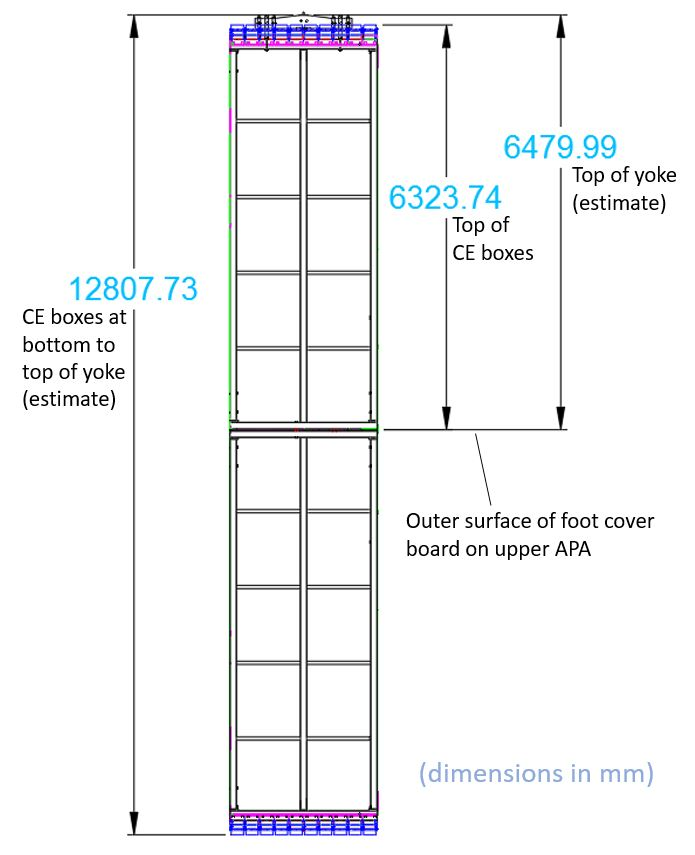
\includegraphics[width=0.8\textwidth]{Dual_APA_dimensioned.jpg} 
\end{dunefigure}

%%%%%%%%%%%%%%%%%%%%%%%%%%%%%%%%%%%
\subsection{Frame and Mesh}
\label{sec:fdsp-apa-frames}

\fixme{Include an image of the subsystem (frame), indicating its parts. Show how the system fits into the overall system (APA).}

The stainless steel frame of the APA (Figure~\ref{fig:tpc_apa_frame}) is 6.06~m long, not counting electronics and mounting hardware, and 2.30~m wide.  It is 76.2~mm thick, made from imperial size 3-in $\times$ 4-in $\times$ 0.120-in wall rectangular tubing.  The cross pieces have a cross-sectional area of 2\,in $\times$ 3\,in, and are connected to edge pieces using joints, as in Figure~\ref{fig:tpc_apa_boltedjointdrawing}.  It is mounted in the cryostat with its long axis vertical; multiple APAs are mounted edge-to-edge to form a continuous plane. An electron deflection technique, described in Section~\ref{sec:apa:electrondiverter}, is used to ensure that electrons drawn towards a joint between two APAs will be deflected to one or the other, and not lost.

\begin{dunefigure}[APA dimensions]{fig:tpc_apa_frame}{An APA showing overall dimensions and main components. }
%\includegraphics[width=0.9\textwidth]{figures/tpc_apa_frame} 
\end{dunefigure}
%\fixme{COMMENT from Justin: it would be good if the dimensions of the upper figure had the same precision as the numbers in the text, i.e. 6.06 m and 2.30 m. (Anne agrees, but we're not updating figures right now.)}

\begin{dunefigure}[APA bolted joint drawing]{fig:tpc_apa_boltedjointdrawing}{A model of the bolted joint.  The holes on the top of the tube are for access to tighten the screws.  The heads actually tighten against the lower hole, inside the tube.}
%\includegraphics[width=0.4\textwidth]{figures/tpc_apa_boltedjointdrawing} 
\end{dunefigure}

A fine mesh screen is glued directly to the steel frame surface, over the frame on both sides.  It creates a uniform ground layer beneath the wire planes.  

The mesh is clamped around the perimeter of the opening and then pulled tight (by opening and closing clamps as needed during the process).  When the mesh is taut, a 25-mm-wide strip is masked off around the opening and glue is applied through the mesh to attach it to the steel.  Although measurements have shown that this gives good electrical contact between the mesh and the frame, a deliberate electrical connection is also made.  Figure~\ref{fig:tpc_apa_fullsizemeshdrawing} depicts the mesh application setup for a full-size ProtoDUNE-SP APA.

\begin{dunefigure}[APA full-size mesh drawing]{fig:tpc_apa_fullsizemeshdrawing}{The mesh clamping jig for the full size APA. }
%\includegraphics[width=0.8\textwidth]{figures/tpc_apa_fullsizemeshdrawing} 
\end{dunefigure}


%%%%%%%%%%%%%%%%%%%%%%%%%%%%%%%%%%%
\subsection{Anchoring Elements and Wire Boards}
\label{sec:fdsp-apa-boards}

\fixme{Include an image of the subsystem (boards), indicating its parts. Show how the system fits into the overall system (APA).}

%%%%%%%%%%%%
\subsubsection{Head Electronics Boards}

At the head end of the APA, stacks of electronics boards (referred to as ``wire boards'') are arrayed to anchor the wires.  They also provide the connection between the wires and the cold electronics.

All APA wires are terminated on the wire boards, which are stacked along the electronics end of the APA frame; see Figure~\ref{fig:tpc_apa_boardstack}. 
Attachment of the wire boards begins with the X plane (innermost). After the X-plane wires are strung top to bottom along each side of the APA frame, they are soldered and epoxied to their wire boards and trimmed. The remaining wire board layers are attached as each layer is wound.  The main CR boards (capacitive-resistive), which provide DC bias and AC coupling to the wires, are attached to the bottom of the wire board stack. 

\begin{dunefigure}[APA board stack]{fig:tpc_apa_boardstack}{Left: View of the APA wire board stack, as seen from the top/side. The wire board layers can be seen at the bottom-left of the illustration, X on the bottom (it doesn't go all the way back, but extends farther forward and has the main CR board attached), followed by U, V, then G (which doesn't go all the way forward, and has its own CR board attached). Right: the same stack viewed from below. }
%\includegraphics[width=0.45\textwidth]{figures/tpc_apa_boardstack_top.jpg}
%\includegraphics[width=0.45\textwidth]{figures/tpc_apa_boardstack_bottom.jpg}
\end{dunefigure}

The outermost G-plane wire boards connect adjacent groups of four wires together, and bias each group through an R-C filter whose components are placed on special CR boards   
that are attached after the wire plane is strung. The X, U and V layers of wires are connected to the CE (housed in boxes mounted on the APA) either directly or through DC-blocking capacitors. The X and U planes have wires individually biased through 50-M$\Omega$ resistors. Electronic components for the X- and U-plane wires are located on a common CR board. 

Mill-Max pins and sockets provide electrical connections between circuit boards within a stack. They are pressed into the circuit boards and are not repairable if damaged. To minimize the possibility of damaged pins, the boards are designed so that the first wire board attached to the frame has only sockets. All boards attached subsequently contain pins that plug into previously mounted boards. This process eliminates exposure of any pins to possible damage during winding, soldering, or trimming processes.

Ten stacks of wire boards are installed across the width of each side along the head of the APA.  The X-layer board in each stack has room for 48 wires, the V layer has 40 wires, the U layer 40 wires and the G layer 48 wires.  Each board stack, therefore, has 176 wires but only 128 signal channels since the G wires are not read out.  
With a total of 20 stacks per APA, this results in 2,560 signal channels per APA and a total of \SI{3520} wires starting at the top of the APA and ending at the bottom.  There is a total of $\sim$23.4 km of wire on the two surfaces of each APA.  Many of the capacitors and resistors that in principle could be on these wire boards are instead
placed on the attached CR boards to improve their accessibility in case of component failure.   Figure~\ref{fig:tpc_apa_electronics_connectiondiagram} depicts the connections between the different elements of the APA electrical circuit. 

At the head end of the APA, the wire-plane spacing is set by the thickness of these wire boards.  The first layer's wires solder to the surface of the first board, the second layer's wires to the surface of the second board, and so on.  For installation, temporary toothed-edge boards beyond these wire boards align and hold the wires until they are soldered to pads on the wire boards.  After soldering, the extra wire is snipped off. 

\begin{dunefigure}[APA wire board connection to electronics]{fig:tpc_apa_electronics_connectiondiagram}{Diagram of the connection between the APA wires, viewed from the APA edge. The set of wire boards within a stack can be seen on both sides of the APA, with the CR board extending further to the right, providing a connection to the cold electronics, which are housed in the boxes at the far right of the figure. }
%\includegraphics[width=0.7\textwidth]{figures/tpc_apa_electronics_connectiondiagram.jpeg}
\end{dunefigure}
%\fixme{this figure could use some labelling}

%%%%%%%%%%%%
\subsubsection{CR Boards}
\label{sec:crboards}

The CR boards carry a bias resistor and a DC-blocking capacitor for each wire in the X and U planes. These boards are attached to the board stacks after fabrication of all wire planes.  Electrical connections to the board stack are made though Mill-Max pins that plug into the wire boards. Connections from the CR boards to the CE are made through a pair of 96-pin Samtec connectors.

Surface-mount bias resistors on the CR boards have resistance of 50\,M$\Omega$ are constructed with a thick film on a ceramic substrate. Rated for 2.0-kV operation, the resistors measure 0.12 $\times$ 0.24 inches. Other ratings include operation from $-$55 to +155 C, 5\% tolerance, and a 100-ppm/C temperature coefficient.
Performance of these resistors at LAr temperature is verified through additional bench testing.

The selected DC-blocking capacitors have capacitance of 3.9\,nF and are rated for 2.0-kV operation. Measuring 0.22 $\times$ 0.25\,inches across and 0.10\,inches high, the capacitors feature flexible terminals to comply with PC board expansion and contraction. They are designed to withstand 1,000 thermal cycles  
between the extremes of the operating temperature range. Tolerance is also 5\%.

In addition to the bias and DC-blocking capacitors for all X- and U-plane wires, the CR board includes two R-C filters for the bias voltages. The resistors are of the same type used for wire biasing except with a resistance of 2\,M$\Omega$. Capacitors are 47\,nF at 2\,kV. Very few choices exist for surface-mount capacitors of this type, and they are exceptionally large. 
Polyester or Polypropylene film capacitors that are known to perform well at cryogenic temperatures are used.


%%%%%%%%%%%%
\subsubsection{Side and Foot Boards}

The boards along the sides and foot of the APA have notches, pins and other location features to hold the wires in the correct position as they wrap around the edge from one side of the APA to the other.

G10 circuit board material is ideal for these side and foot boards due to its physical properties alone, but it has an additional advantage: a number of hole or slot features in the edge boards provide access to the underlying frame.  In order that these openings are not covered by wires, the sections of wire that would go over the openings are replaced by traces on the boards.  After the wires are wrapped, the wires over the opening are soldered to pads at the ends of the traces, and the section of wire between the pads is snipped out (Figure~\ref{fig:tpc_apa_sideboardmodel}).  These traces are easily and economically added to the boards by the many commercial fabricators who make circuit boards. 

\begin{dunefigure}[APA side board model]{fig:tpc_apa_sideboardmodel}{Model of board with wires showing how traces connect wires around openings in the side boards.  The wires are wound straight over the openings, then soldered to pads at the ends of the traces.  After soldering the sections between the pads are trimmed away.}
%\includegraphics[width=0.9\textwidth]{figures/tpc_apa_sideboardmodel} 
\end{dunefigure}


\begin{dunefigure}[APA side board photo]{fig:tpc_apa_sideboardphoto}{Boards with injection molded tooth strips glued on.  The left shows an end board with teeth for fixing the position of the longitudinal wires.  The teeth there form small notches. The right is a side board for fixing the position of the angled wires where the wires are angled around a pin. (These boards are prototype test pieces and are not used in the production APAs.)}
%\includegraphics[width=0.7\textwidth]{figures/tpc_apa_sideboardphoto} 
\end{dunefigure}

The placement of the angled wires are fixed by pins 
as shown in the right-hand picture of Figure~\ref{fig:tpc_apa_sideboardphoto}.  The wires make a partial wrap around the pin as they change direction from the face of the APA to the edge.  The X- and G-plane wires are not pulled to the side so they cannot be pulled against a pin.  Their positions are fixed 
by teeth with slots, as shown in the left-hand picture in Figure~\ref{fig:tpc_apa_sideboardphoto}. 
	
The polymer used for the strips is Vectra e130i (a trade name for 30$\%$ glass filled liquid crystal polymer or LCP). It retains its strength at cryogenic temperature and has a CTE similar enough to G10 that differential expansion/contraction is not a problem.

%%%%%%%%%%%%
\subsubsection{Glue and Solder}
The ends of the wires are soldered to pads on the edges of the wire boards.  Solder provides both an electrical connection and a physical anchor to the wires.  As an additional physical anchor, roughly 10~mm of the wires are glued near the solder pads.  For example, in Figure~\ref{fig:tpc_apa_sideboardphoto}, in addition to soldering the wires on the pads shown in the left-hand photograph, an epoxy bead is applied on the wires in the area between the solder pads and the injection-molded tooth strips.

Gray epoxy 2216 by 3M is used for the glue.  It is strong, widely used (therefore much data is available), and it retains good properties at cryogenic temperatures.  A 62$\%$ tin, 36$\%$ lead and 2$\%$ silver solder was chosen.  A eutectic mix (63/37) is the best of the straight tin/lead solders but the 2$\%$ added silver gives better creep resistance.

%%%%%%%%%%%%%%%%%%%%%%%%%%%%%%%%%%%
\subsection{Wires}
\label{sec:fdsp-apa-wires}

Beryllium copper (CuBe) wire is known for its high durability and yield strength. It is composed of $\sim$98$\%$ copper, 1.9$\%$ beryllium, and a negligible amount of other elements. The APA wire has a diameter of 150$\mu$m (.006~in), and is strung in varying lengths across the APA frame. Three key properties for its usage in the APA are: low resistivity, high tensile or yield strength, and coefficient of thermal expansion suitable for use with the APA's stainless steel frame.

Tensile strength of the wire describes the wire-breaking stress (see Table~\ref{tab:wire}).  The yield strength is the stress at which the wire starts to take a permanent (inelastic) deformation, and is the important limit stress for this case, though most specifications give tensile strength.  Fortunately, for the CuBe alloys of interest, the two are fairly close to each other.  Based on the tensile strength of wire purchased from Little Falls Alloy (over 1,380~MPa or 200,000~psi), the yield strength is greater than 1,100~MPa.  Given that the stress while in use is around 280~MPa, this leaves a comfortable margin.

The coefficient of thermal expansion (CTE) describes how material expands and contracts with changes in temperature.  The CTEs of CuBe alloy and 304 stainless steel are very similar.  Integrated down to 87~K, they are 2.7e-3 for stainless and 2.9e-3 for CuBe~\cite{cryo-mat-db}.
Since the wire contracts slightly more than the frame during cool-down the wire tension increases.  If it starts at 5~N, the tension rises to about 5.5~N when everything is cool.  

The change in wire tension during cool-down could also be a concern.  In the worst case, the wire
 cools quickly to 87\,K before any significant cooling of the frame  -- a realistic case because of the differing thicknesses.  In the limiting case, with complete contraction of the wire and none in the frame, the tension would be expected to reach $\sim$11.7 N.  This is still well under the $\sim$20 N yield tension.
In practice, the cooling will be done gradually to avoid this tension spike as well as other thermal shock to the APA.

\begin{dunetable}[CuBe wire tensile strength and CTE]{lr}{tab:wire}{Tensile strength and coefficient of thermal expansion (CTE) of beryllium copper (CuBe) wire.}
Parameter & Value \\ \toprowrule
Tensile Strength (from property sheets) (psi) & 208,274 \\ \colhline
Tensile Strength (from actual wire) (psi) & 212,530 \\ \colhline
CTE of CuBe, integrated to 87 K (m/m) & 2.9e-3 \\ \colhline
CTE of 304 stainless steel, integrated to 87 K (m/m) & 2.7e-3 \\
\end{dunetable}



%%%%%%%%%%%%%%%%%%%%%%%%%%%%%%%%%%%%
\subsection{Quality Assurance}
\label{sec:fdsp-apa-qa}

\fixme{Ideas from the QA plan - topics to address}

Work processes: ensure proper training materials for and training of designers, fabricators, etc. 

Design validation: APA has had design reviews, and is prototyped in ProtoDUNE-SP...

Acceptance Testing of procured items? 

Lessons learned 

Documents and records for all these things.


%%%%%%%%%%%%%%%%%%%%%%%%%%%%%%%%%%%%%%%%%%%%%%%%%%%%%%%%%%%%%%%%%%%%
\section{Production and Assembly}
\label{sec:fdsp-apa-prod-assy}


%%%%%%%%%%%%%%%%%%%%%%%%%%%%%%%%%%%
\subsection{Production Plan}
\label{sec:fdsp-apa-prod-plan}


%%%%%%%%%%%%%%%%%%%%%%%%%%%%%%%%%%%
\subsection{Facility Plans}
\label{sec:fdsp-apa-facility}


%%%%%%%%%%%%%%%%%%%%%%%%%%%%%%%%%%%
\subsection{Wire Winding Machine}
\label{sec:fdsp-apa-winding}


%%%%%%%%%%%%%%%%%%%%%%%%%%%%%%%%%%%
\subsection{Tooling}
\label{sec:fdsp-apa-tooling}


%%%%%%%%%%%%%%%%%%%%%%%%%%%%%%%%%%%
\subsection{Assembly Procedures, Travelers, and Documentation}
\label{sec:fdsp-apa-assy}




%%%%%%%%%%%%%%%%%%%%%%%%%%%%%%%%%%%%%%%%%%%%%%%%%%%%%%%%%%%%%%%%%%%%
\section{Interfaces}
\label{sec:fdsp-apa-intfc}

 

\fixme{It would be nice to coordinate with the interface documents; email to Jack F sent 12/20}

\fixme{Include an image of each interface in appropriate section.}

%%%%%%%%%%%%%%%%%%%%%%%%%%%%%%%%%%
\subsection{LBNF Cryostat and Detector Support Structure}
\label{sec:fdsp-apa-intfc-lbnf-dss}


%%%%%%%%%%%%%%%%%%%%%%%%%%%%%%%%%
\subsection{Photon Detection System}
\label{sec:fdsp-apa-intfc-pds}


%%%%%%%%%%%%%%%%%%%%%%%%%%%%%%%%%
\subsection{TPC Electronics}
\label{sec:fdsp-apa-intfc-elec}




%%%%%%%%%%%%%%%%%%%%%%%%%%%%%%%%%%%%%%%%%%%%%%%%%%%%%%%%%%%%%%%%%%%%
\section{Installation, Integration and Commissioning}
\label{sec:fdsp-apa-install}

%%%%%%%%%%%%%%%%%%%%%%%%%%%%%%%%%%%
\subsection{Transport and Handling}
\label{sec:fdsp-apa-install-transport}


%%%%%%%%%%%%%%%%%%%%%%%%%%%%%%%%%%%
\subsection{Integration with PDS and TPC Electronics}
\label{sec:fdsp-apa-install-pds-elec}


%%%%%%%%%%%%%%%%%%%%%%%%%%%%%%%%%%%
\subsection{Calibration}
\label{sec:fdsp-apa-install-calib}




%%%%%%%%%%%%%%%%%%%%%%%%%%%%%%%%%%%%%%%%%%%%%%%%%%%%%%%%%%%%%%%%%%%%
\section{Quality Control}
\label{sec:fdsp-apa-qc}

%%%%%%%%%%%%%%%%%%%%%%%%%%%%%%%%%%%%%
\subsection{Protection and Assembly (Local)}
\label{sec:fdsp-apa-qc-local}


%%%%%%%%%%%%%%%%%%%%%%%%%%%%%%%%%%%%%%%
\subsection{Post-factory Installation (Remote)}
\label{sec:fdsp-apa-qc-remote}



%%%%%%%%%%%%%%%%%%%%%%%%%%%%%%%%%%%%%%%%%%%%%%%%%%%%%%%%%%%%%%%%%%%%
\section{Safety}
\label{sec:fdsp-apa-safety}

\fixme{Points taken from doc 2145, dune mgmt plan}

IPO provides an installation resource where either critical safety issues exist (for example,  crane	
operation) or effort is needed which spans all	detector elements (material transport). What's required for APA?

Is there a Detector Integration, Testing and Installation (DITI) Group with safety being one aspect of their responsibility?

Slow controls safety system -- is this relevant?

%%%%%%%%%%%%%%%%%%%%%%%%%%%%%%%%%
% add subsections and labels if needed \subsection{}
%\label{sec:fdsp-apa-safety-}


%%%%%%%%%%%%%%%%%%%%%%%%%%%%%%%%
%\subsection{}
%\label{sec:fdsp-apa-safety}



%%%%%%%%%%%%%%%%%%%%%%%%%%%%%%%%%%%%%%%%%%%%%%%%%%%%%%%%%%%%%%%%%%%%
\section{Organization and Management}
\label{sec:fdsp-apa-org}

%%%%%%%%%%%%%%%%%%%%%%%%%%%%%%%%%%%%%
\subsection{APA Consortium Organization}
\label{sec:fdsp-apa-org-consortium}

\fixme{I asked Maxine about standardized org charts for each consortium. It would be nice to have these. Anne}

%%%%%%%%%%%%%%%%%%%%%%%%%%%%%%%%%%%%%%
\subsection{Planning Assumptions}
\label{sec:fdsp-apa-org-assmp}


%%%%%%%%%%%%%%%%%%%%%%%%%%%%%%%%%%%%%%
\subsection{WBS and Responsibilities}
\label{sec:fdsp-apa-org-wbs}

%%%%%%%%%%%%%%%%%%%%%%%%%%%%%%%%%%%%%%%
\subsection{High-level Cost and Schedule}
\label{sec:fdsp-apa-org-cs}

















